\section{Valószínűségi következtetés}

\subsubsection{Bizonytalanság}

Jelölje $A_t$ azt a műveletet, hogy $t$ perccel a vonat indulása előtt
elindulunk a pályaudvarra. $A_t$-vel időben odaérünk? A következő
problémák lépnek fel:
\begin{itemize}
    \item részlegesen megfigyelhető környezet (utak állapota, más sofőrök
        terve, stb.)
    \item zajos észlelések (Útinfo, DKV applikáció jelzései)
    \item a művelet kimenelének bizonytalansága (lapos gumi, stb.)
    \item a közlekedés modellezésének és előrejelzésének hatalmas bonyolultsága
\end{itemize}

Logikai megközelítésben
A probléma logikai megközelítése:
\begin{itemize}
    \item kockázat elutasítása: "$A_{25}$ esetén odaérek"
    \item pontos megfogalmazás (túl határozatlan döntéshozatalhoz) "$A_{25}$-tel
        odaérek, ha nincs útközben baleset, útfelújítás, és nem történik addig
        a kocsival semmi, stb."
\end{itemize}

$A_{120}$ biztosan elég (még gyalog is odaértek), de senki nem akar ennyi időt
az állomáson tölteni.

\subsubsection{Bizonytalanság kezelésének módszerei}

\begin{itemize}
    \item Alapértelmezett vagy nem-monoton logika
        \begin{itemize}
            \item feltesszük, hogy a kocsinak nem lyukad ki a gumija
            \item feltesszük, hogy $A_{25}$ elég, hacsak nem mond ellent a
                nyilvánvaló tényeknek
            \item Mely feltételek ésszerűek? Hogyan kezelhetjük az
                ellentmondásokat?
        \end{itemize}

    \item Szabályok tapasztalati tényezőkkel
        \begin{itemize}
            \item $A_{25} \Rightarrow_{0.3}$ Időben kiér az állomásra
            \item locsol $\Rightarrow_{0.99}$ vizes a fű
            \item vizes a fű $\Rightarrow_{0.7}$ esett az eső
            \item szabályok kombinálása: A locsol következménye az esett az eső?
        \end{itemize}

    \item Valószínűség
        \begin{itemize}
            \item A nyilvánvaló tények mellett $A_{25}$ esetén 4\% eséllyel jutok el
                időben az állomásra.
        \end{itemize}

    \item Fuzzy logika
        \begin{itemize}
            \item igazság foka (és nem bizonytalanság)
            \item "a fű vizes" értéke 0.2
                \begin{itemize}
                    \item nem "100 esetben 20-szor vizes a fű"
                    \item hanem "enyhén vizes a fű"
                \end{itemize}
        \end{itemize}
\end{itemize}

\subsubsection{Valószínűség}

Valószínűségi feltételek összegzik a
\begin{itemize}
    \item lustaságot: túl sok munkát jelent az ok és okozat teljes
        eseményhalmazának felsorolása
    \item elméleti tudatlanságot: a tudományterület elmélete nem teljes
    \item gyakorlati tudatlanságot: nem végezhető el az összes vizsgálat
\end{itemize}

Észlelések alkotják a tényt/tényállást
\begin{itemize}
    \item a kihúzott lap pikk ász (1/52 valószínűséggel - lap megnézése nélkül)
    \begin{itemize}
        \item megnézéssel 0 vagy 1 valószínűséggel
    \end{itemize}
    \item mielőtt a tények birtokába jutunk előzetes/a priori valószínűség
    \item tények birtokában utólagos/a posteriori/feltételes valószínűség
\end{itemize}

A valószínűségek személyes meggyőződésekhez/hiedelmekhez kapcsolódhatnak.

\subsubsection{Döntések bizonytalanság mellett}

Tekintsük a következő feltételezéseket:
\begin{itemize}
    \item $P(A_{25} \text{-tel időben odaérek|\ldots}) = 0.04$
    \item $P(A_{30} \text{-cal időben odaérek|\ldots}) = 0.23$
    \item $P(A_{75} \text{-tel időben odaérek|\ldots}) = 0.74$
    \item $P(A_{120} \text{-szal időben odaérek|\ldots}) = 0.999$
\end{itemize}

Ekkor az, hogy melyik műveletet választjuk függ a személyes preferenciáktól:
lekésett vonat, várakozás, \ldots.

\begin{itemize}
    \item Hasznosságelmélet: preferenciák ábrázolása és felhasználása
    \item Döntéselmélet $=$ hasznosságelmélet  $+$ valószínűség
\end{itemize}

\subsubsection{Valószínűségszámítás alapjai}

\begin{definicio}
    Elemi események, elemi események halmaza.
    Legyen $\Omega$ az elemi események egy halmaza (pl. a kockadobás hat
    kimenetele).  Ekkor  $\omega \in \Omega$ egy elemi esemény, egy lehetséges
    világ. Az elemi események kölcsönösen kizárják egymást.

    Minden elemi eseményhez rendelhető egy valószínűség: \[
        0 \le P(\omega) \le 1
    ,\] ahol $\sum P(\omega) = 1$.
\end{definicio}

\begin{tetel}
    Ha egy  $A$ esemény adott elemei események uniója, akkor az $A$
    valószínűsége az adott elemi események valószínűségének összege.
\end{tetel}

\begin{definicio}
    A valószínűségi változó egy függvény, mely az elemi eseményekhez
    egy értéket (rendszerint valós, vagy logikai) rendel, például
    $\text{páratlan}(1) = \text{igaz}$, vagy $\text{páros}(3) = \text{hamis}$.

    A $P$ bármely $X$ valószínűségi változóhoz valószínűségi eloszlást rendel:
    \[
        P(X = x_i) = \sum_{\omega : X(\omega) = x_i} P(\omega)
    .\]
\end{definicio}

A valószínűségeket azért használjuk, mert a logikailag összekapcsolódó
események valószínűségei is összekapcsolódnak: \[
    P(a \lor b) = P(a) + P(b) - P(a \land b)
.\]

\subsubsection{Állítások}

Állításnak azt tekintjük, amikor egy esemény (elemi események halmaza)
teljesül.

Legyen $A$ és $B$ két véletlen változó. Ekkor
\begin{itemize}
    \item $a$ esemény = azon elemi események halmaza, ahol $A(\omega) =$ igaz
    \item $\lnot a$ esemény = azon elemi események halmaza, ahol $A(\omega) =$ hamis
    \item $a \land b$ esemény = azon elemi események halmaza, ahol $A(\omega)
        =$ igaz és $B(\omega) =$ igaz
\end{itemize}

MI alkalmazásokban az elemi eseményeket a valószínűségi változók értékei
határozzák meg.  Pl. az elemi események halmaza az értékkészletek
Descartes-szorzata.

Logikai változók esetén az elemi esemény egy nulladrendű interpretáció.

Egy állítás elemi állítások diszjunkciója.

\begin{tetel}
    Állítások szintaxisa.

    \begin{itemize}
        \item Ítéletlogikai vagy logikai valósínűségi változó
            \begin{itemize}
                \item Lyuk (lyukas a fogam?)
                \item "Lyuk = igaz" egy állítás, leírható lyukas alakban is
            \end{itemize}
        \item Diszkrét valószínűségi változó (véges vagy végtelen)
            \begin{itemize}
                \item az Időjárás a (napos, esős, felhős és havas) egyike
                \item "Időjárás = esős" egy állítás
                \item az értékeknek egymást kizárónak kell lenniük, és ki kell
                    adniuk az összes lehetőséget
            \end{itemize}
        \item Folytonos valószínűségi változó (korlátos vagy nem korlátos)
            \begin{itemize}
                \item "Hőmérséklet = 21.6" vagy "Hőmérséklet < 22.1" állítások
            \end{itemize}
    \end{itemize}
\end{tetel}

\begin{tetel}
    Állítások bármilyen logikai kombinációja újabb állítást ad.
\end{tetel}

\subsubsection{Priori -- előzetes valószínűség}

A priori állítások előzetes, vagy feltétel nélküli valószínűsége. Azt a
meggyőződési mértéket jelenti, amely bármely más információ hiányában
az állításhoz kapcsolható. Pl.: \[
    P(\text{lyukas}) = 0.1, \quad\quad P(\text{Időjárás=napos}) = 0.73
.\]

A valószínűségi eloszlás értéket rendel minden lehetséges értékadáshoz. Pl.: \[
    P(\text{Időjárás}) = (0.73; 0.1; 0.07; 0.1)
.\] Ez a mennyiség normalizált, az egyes eshetőségek összege 1.

Együttes valószínűségi eloszlás: véletlen változóhalmaz összes lehetséges
kombinációjának valószínűsége.

\begin{center}
    $P(\text{Időjárás}, \text{Lyuk}) = $
    \begin{tabular}{|l|c|c|c|c|}
        \hline
        Időjárás & napos & esős & felhős & havas \\\hline
        Lyuk = igaz     & 0.144     & 0.02  & 0.016     & 0.02 \\\hline
        Lyuk = hamis    & 0.576     & 0.08  & 0.064     & 0.08 \\\hline
    \end{tabular}
\end{center}

\subsubsection{Folytonos változók valószínűsége}

A lehetséges értékek száma végtelen, így táblázatban nem foglalható össze.
Annak valószínűsége, hogy egy valószínűségi változó egy adott $x$ értéket
vesz fel, általában $x$ egy paraméterezett függvényeként definiálható. Pl. \[
    P(\text{Hőmérséklet} = x) = \bigcup_{i=18}^{26}(x)
\] -- azaz egyenletes eloszlású 18 és 26 C$^{\circ}$ között.

$P(X = 20.5) = 0.125$ értelmezése: \[
    \lim_{\text{d}x\to 0} \frac{P(20.5 \le X \le 20.5 + \text{d}x)}{\text{d}x}
    = 0.125
.\]

\subsection{Bayes hálók, Bayes tétel}

\begin{tetel}
    A Bayes-tétel: \[
        P(b|a) = \frac{P(a|b)P(b)}{P(b)}
    .\]
\end{tetel}

\begin{tetel}
    A Bayes-tétel általános eloszlásokra
    \[
        P(Y|X) = \frac{P(X|Y)P(Y)}{P(X)}
    .\]
\end{tetel}

\begin{definicio}
    A Bayes-hálók egy a bizonytalanság esetén használható tudás-reprezentációs
    módszer adatstruktúrája. A Bayes-hálók alkalmasak változók közötti függőség
    leírásához, és bármely együttes valószínűség-eloszlás függvény tömör
    megadásához.

    A Bayes-háló egy irányított gráf, amelyben minden csomóponthoz számszerű
    valószínűségi információk vannak csatolva. A teljes megadás a következő:

    \begin{enumerate}
        \item A háló csomópontjait valószínűségi változók egy halmaza alkotja.
            A változók lehetnek diszkrétek, vagy folytonosak.
        \item Irányított élek (nyilak) egy halmaza összeköt bizonyos
            csomópontpárokat. Ha létezik nyíl az $X$ csomóponttól
            az $Y$ csomópontig, azt mondjuk, $X$ szülője az $Y$-nak.
        \item Minden $X_i$ csomóponthoz tartozik egy $P(X_i|\text{Szülők}(X_i)$
            feltételes valószínűségi eloszlás, ami számszerűen megadja a szülők
            hatását a csomóponti változóra.
        \item A gráf nem tartalmaz irányított kört (azaz irányított, körmentes
            gráf).
    \end{enumerate}

    \begin{figure}[H]
        \centering
        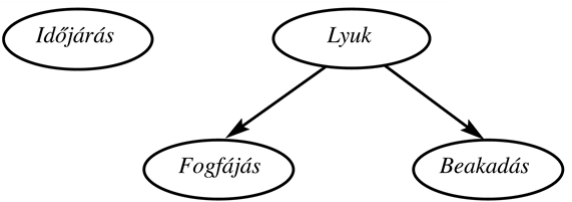
\includegraphics[width=0.8\textwidth]{bayes1}
        \caption{Egy egyszerű Bayes-háló, amelyben az Időjárás független a
            többi három változótól, a Fogfájás és Beakadás pedig feltételesen
            függetlenek a Lyuk ismeretében}
        \label{fig:bayes1}
    \end{figure}

    \begin{figure}[H]
        \centering
        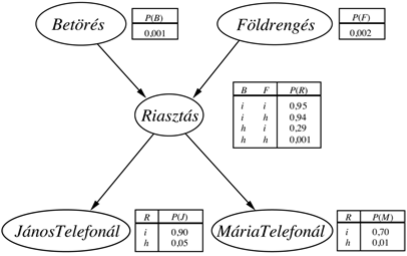
\includegraphics[width=0.8\textwidth]{bayes2}
        \caption{Egy tipikus Bayes-háló, amely a topológiát és a
            feltételes valószínűségi táblákat (FVT) is mutatja.}
        \label{fig:bayes2}
    \end{figure}
\end{definicio}

\subsection{Feltételes valószínűség számítása}

\subsubsection{Feltételes valószínűség}

Ha az ágens bizonyos tények birtokába jut a korábban ismeretlen, a tartományra
jellemző véletlen változóra vonatkozóan, akkor a priori valószínűségek nem
használhatóak. Például \[
    P(\text{lyukas} | \text{fogfájás}) = 0.8
\]  esetén
\begin{itemize}
    \item adott, hogy a betegnek fáj a foga; ezt és csak ezt tudjuk
    \item nem arról van szó, hogy "ha fáj a foga, akkor 80\% eséllyel lyukas"
    \item hanem "ha fáj a foga és semmilyen más információnk nincs, akkor 80\%
        eséllyel lyukas"
\end{itemize}

\subsubsection{Képlet}

A feltételes valószínűség definíciója (ha $P(b) \neq 0$) \[
    P(a|b) = \frac{P(a \land b)}{P(b)}
.\]

\subsubsection{Szorzat szabály}

A szorzat szabály egy alternatív megfogalmazás:
\[
    P(a \land b) = P(a|b)P(b) = P(b|a)P(a)
.\]

\subsubsection{Láncszabály}

A szorzatszabály többszöri alkalmazásával kapjuk meg a láncszabályt:
\[
    P(X_1, \ldots, X_n) =
    P(X_n | X_1, \ldots, X{n-1}) \cdot P(X_1 | X_1, \ldots, X{n-1})
    = \prod^n_{i=1}P(X_i | X_1, \ldots, X_{i-1})
.\]

\subsubsection{Feltételes valószínűség kiszámítása}

\begin{align*}
    P(\text{lyuk}|\text{fogfájás}) &= \frac{P(\text{lyuk}) \land
        \text{fogfájás}}{P(\text{fogfájás)}} =
        \frac{0.108 + 0.012}{0.018+0.012+0.016+0.064} = 0.6 \\
    P(\lnot \text{lyuk}|\text{fogfájás}) &= \frac{P(\lnot \text{lyuk}) \land
        \text{fogfájás}}{P(\text{fogfájás)}} =
        \frac{0.016 + 0.064}{0.018+0.012+0.016+0.064} = 0.4
\end{align*}
